\part{Dérivation}

\underline{Motivation}:

{
\begin{wrapfigure}{l}{3cm}
	\centering
	\begin{asy}
		import three;

		size(3cm);
		settings.render=0;
		settings.prc=false;
		currentprojection = obliqueZ;

		draw(unitbox);
		draw(shift(1.1Z + 0.05X) * (O -- X), Arrows3(TeXHead2));
		draw(shift(1.1Z + 0.05Y) * (O -- Y), Arrows3(TeXHead2));
		draw(shift(1.1X + 0.05Z) * (O -- Z), Arrows3(TeXHead2));

		label("$x$", (X/2) + (1.1Z + 0.05X), align=S);
		label("$y$", (Y/2) + (1.1Z + 0.05Y), align=W);
		label("$z$", (Z/2) + X, align=SE);
	\end{asy}
\end{wrapfigure}

\begin{align*}
	&S(x,y,z) = 2(xy + xz + yz)\\
	&V(x,y,z) = xyz
\end{align*}

On cherche à minimiser $S$ avec la contrainte $V = 1$.

Soit $f : \begin{array}{rcl}
	\left( \R_*^+ \right)^2 &\longrightarrow& \R \\
	(x,y) &\longmapsto& S\left( x,y,\frac{1}{xy} \right) = 2\left( xy + \frac{1}{y} + \frac{1}{x} \right).
\end{array}$

On cherche $(a,b) \in \left( \R^+_* \right)^2$ tel que \[
	\forall (x,y) \in (\R^+_*), f(x,y) \ge f(a,b).
\]
}

\begin{defn}
	Soit $f: U \to \R$ où $U$ est un ouvert de $\R^2$. Soit $(a,b) \in U$.
	\vspace{2mm}

	Si $\lim_{x \to a} \frac{f(x,b) - f(a,b)}{x - a} \in \R$, alors on dit que $f$ a une dérivée partielle suivant $x$ en $(a,b)$ et cette limite est notée \[
		\partial f_1(a,b) = \frac{\partial f}{\partial x}(a,b).
	\]

	Si $\lim_{y \to b} \frac{f(a,y) - f(a,b)}{y - b} \in \R$, alors on dit que $f$ a une dérivée partielle suivant $y$ et la limite est notée \[
		\partial f_2(a,b) = \frac{\partial f}{\partial y}(a,b).
	\]
\end{defn}

\begin{exm}
	\begin{enumerate}
		\item $f: (x,y) \mapsto xy + x - y$.

			\begin{align*}
				&\frac{\partial f}{\partial x} : (x,y) \mapsto y + 1,\\
				&\frac{\partial f}{\partial y} : (x,y) \mapsto x - 1.
			\end{align*}

		\item $f: (x,y) \mapsto xy + \frac{1}{y}+ \frac{1}{x}$.

			\begin{align*}
				&\frac{\partial f}{\partial x}: (x,y) \mapsto y - \frac{1}{x^2},\\
				&\frac{\partial f}{\partial y}: (x,y) \mapsto x - \frac{1}{y^2}.
			\end{align*}

		\item Trouver $f$ telle que $\begin{cases}
				(1): \qquad \frac{\partial f}{\partial x}=y,\\[2mm]
				(2): \qquad \frac{\partial f}{\partial y} = x.
			\end{cases}$

			D'après $(1)$ : \[
				\forall (x,y), \exists C(y) \in \R, f(x,y) = xy + C(y)
			\] et donc \[
				\frac{\partial f}{\partial y}(x,y) = x + C'(y)
			\] donc $C'(y) = 0$ et donc $C$ est constante.

		\item Trouver $f$ telle que $\begin{cases}
			\frac{\partial f}{\partial x} = -y,\\[2mm]
			\frac{\partial f}{ƒ\partial y} = x.
		\end{cases}$

		Ce n'est pas possible !
	\end{enumerate}
\end{exm}

\begin{defn}~\\
	\begin{minipage}{\linewidth}
		\begin{wrapfigure}{r}{4cm}
			\centering
			\vspace{-5mm}
			\begin{asy}
				import three;
				import graph3;
				size(4cm);

				settings.render = 0;
				settings.prc = false;
				currentprojection = obliqueX;

				draw(O -- X, Arrow3(TeXHead2));
				draw(O -- Y, Arrow3(TeXHead2));
				draw(O -- Z, Arrow3(TeXHead2));

				triple f(real x, real y, real z = 0) { return (x,y,cos(x - 0.5) * cos(y - 0.5)/1.2 + 0.15); }

				real inc = 1 / 5;

				for(real x = 0; x <= 1; x += inc) {
					draw(graph(
						new real(real t) { return x; }, // x
						new real(real y) { return y; }, // y
						new real(real y) { return f(x,y).z; }, // z
						0, 1
					), gray);
				}

				for(real y = 0; y <= 1; y += inc) {
					draw(graph(
						new real(real x) { return x; }, // x
						new real(real t) { return y; }, // y
						new real(real x) { return f(x,y).z; }, // z
						0, 1
					), gray);
				}

				path3 path1 = (0.8, 0.2, 0) .. (0.5, 0.5, 0) .. (0.3, 0.7, 0);
				path3 path2 = f(0.8, 0.2, 0) .. f(0.5, 0.5, 0) .. f(0.3, 0.7, 0);
				path3 d = (0.2, 0.3, 0) .. (0.3, 0.4, 0) .. (0.2, 0.7, 0) .. (0.8, 0.9, 0) .. (0.6, 0.2, 0) .. cycle;

				draw(path1, red, Arrow3(TeXHead2));
				draw(path2, red, Arrow3(TeXHead2, position=0.8));

				dot((0.5, 0.5, 0));
				dot(f(0.5, 0.5, 0));
				draw((0.5, 0.5, 0) -- f(0.5, 0.5, 0), dashed);
				draw(d);

				label("$w$", (0.3, 0.7, 0), red, align=SE);
				label("$U$", (0.8, 0.9, 0), align=SE);
			\end{asy}
		\end{wrapfigure}

		Soit $f: U \to \R$ où $U$ est un ouvert. Soit $(a,b) \in U$. Soit $w = (w_1, w_2) \in \R^2$.

		Si 
		\[
			\lim_{t\to 0} \frac{f(a + tw_1, b + tw_2) - f(a,b)}{t}
		\] existe et est réelle, alors on dit que $f$ a une dérivée dans la direction de $w$ et la limite est notée \[
			\mathrm{d}f(w)\,(a,b) = D_w(f)\,(a,b).
		\]
	\end{minipage}
\end{defn}

\begin{exm}
	\begin{align*}
		f: \left( \R_*^+ \right)^2 &\longrightarrow \R \\
		(x,y) &\longmapsto xy+\frac{1}{x}+\frac{1}{y}.
	\end{align*}

	On pose $(a,b) = (1,2)$, $w = (w_1, w_2) = (1,1)$.
	\begin{align*}
		\frac{f(1+t, 2+t) - f(1,2)}{t} &= \frac{1}{t} \left( (1+t)(2+t) + \frac{1}{1+t} + \frac{1}{2+t} - 3 - \frac{1}{2} \right) \\
		&= \frac{1}{t}\left(\cancel 2 + 3t + \po(t) + \cancel 1 - t + \po(t) + \frac{1}{2}\left( \cancel 1 - \frac{t}{2} + \po(t) \right) - \cancel3 - \cancel{\frac{1}{2}} \right) \\
		&= \frac{1}{t} \left( \frac{7}{4} t + \po(t) \right)  \\
		&= \frac{7}{4} + \po(1) \tendsto{t \to 0} \frac{7}{4}. \\
	\end{align*}

	Donc, \[
		\mathrm{d}f(1,1)\,(1,2) = \frac{7}{4}.
	\]
\end{exm}

\begin{rmk}~\\
	\begin{figure}[H]
		\centering
		\begin{asy}
			import solids;
			import graph;
			size(5cm);

			settings.render = 0;
			settings.prc = false;

			path3 par = graph(
				new real(real x) { return x; },
				new real(real x) { return 0; },
				new real(real x) { return x^2; },
				0,3);
			revolution r = revolution(par, axis=Z);

			path3 par2 = graph(
				new real(real x) { return x; },
				new real(real x) { return 0; },
				new real(real x) { return x^2; },
				-3,3);

			draw(r,1,longitudinalpen=nullpen);
			draw(r.silhouette());

			draw((-4, 0, -1) -- (-4, 0, 10) -- (4, 0, 10) -- (4, 0, -1) -- cycle, red);
			draw(par2, deepred);

			draw((4,4.5) -- (7, 4.5), black+0.5mm, Arrow(TeXHead));

			path par2d = graph(new real(real x) { return x^2; }, -3, 3);
			draw(shift((11, 0)) * par2d, deepred);

			dot(O);
			dot((11, 0));
		\end{asy}
	\end{figure}
\end{rmk}


%todo ajouter théorème-définition
\begin{thm}
	Soit $f : U \to \R$, $(a,b) \in U$. On suppose que $\frac{\partial f}{\partial x}$ et $\frac{\partial f}{\partial y}$ existent en $(a,b)$ et sont {\bfseries continues} en $(a,b)$. Alors,
	\begin{align*}
		&\forall (h, k) \in \R^2 \text{ tel que } (a +h, b + k) \in U,\\
		&f(a+ h, b + k) = f(a,b) + h \frac{\partial f}{\partial x}(a,b) + k \frac{\partial f}{\partial y}(a,b) + \po_{(h,k)\to (0,0)}\big(\|(h,k)\|\big).
	\end{align*}

	On dit que $f$ est de classe $\mathcal{C}^1$ si $\frac{\partial f}{\partial x}$ et $\frac{\partial f}{\partial y}$ existent et sont continues.

	\qed
\end{thm}

\begin{rmk}
	En physique, cette formule correspond à : \[
		\mathrm{d}f = \frac{\partial f}{\partial x}\mathrm{d}x + \frac{\partial f}{\partial y} \mathrm{d}y.
	\] En effet :
	\begin{align*}
		\mathrm{d}f &= f(x+ \mathrm{d}x, y + \mathrm{d}y) - f(x,y) \\
		&= \frac{\partial f}{\partial x} \mathrm{d}x + \frac{\partial f}{\partial y} \mathrm{d}y.
	\end{align*}
\end{rmk}

\begin{prop}
	Soit $f: U \to \R$ de classe $\mathcal{C}^1$ en $(a,b) \in U$. Alors, \[
		\forall w = (w_1, w_2) \in \R^2, \mathrm{d}f(w)\,(a,b) = w_1 \frac{\partial f}{\partial x}(a,b) + w_2 \frac{\partial f}{\partial y}(a,b).
	\]
\end{prop}

\begin{prv}
	Soit $w = (w_1, w_2) \in \R^2$. Soit $t \in \R^*$.
	\begin{align*}
		\frac{1}{t}\big(f(a + tw_1, b + tw_2) - f(a,b)\big)
		&= \frac{1}{t} \left( tw_1 \frac{\partial f}{\partial x}(a,b) + tw_2 \frac{\partial f}{\partial y}(a,b) + \po_{t \to 0}\big(\|tw\|\big) \right) \\
		&= w_1 \frac{\partial f}{\partial x}(a,b) + w_2 \frac{\partial f}{\partial y}(a,b) + \po_{t\to 0}(1) \\
		&\tendsto{t\to 0} w_1 \frac{\partial f}{\partial x}(a,b) + w_2\frac{\partial f}{\partial y}(a,b).
	\end{align*}
\end{prv}


\begin{defn}
	Avec les hypothèses précédentes, en posant \[
		\nabla f(a,b) = \left( \frac{\partial f}{\partial x}(a,b), \frac{\partial f}{\partial y}(a,b) \right) 
	\]on obtient \[
		\mathrm{d}f(w)\,(a,b) = \left<w  \mid \nabla f(a,b) \right>
	\] où $\left<\cdot|\cdot \right>$ est le produit scalaire.

	Le vecteur $\nabla f(a,b)$ est appelé \underline{gradient de $f$ en $(a,b)$}.

	Le développement limité à l'ordre 1 de $f$ devient \[
		f\big((a,b)+w\big) = f(a,b) + \left<w \mid \nabla f(a,b) \right> + \po_{w\to 0}(\|w\|)
	\]
\end{defn}

\begin{prop}
	Soit $f : U \to \R$ de classe $\mathcal{C}^1$.

	\begin{figure}[H]
    \centering
    \incfig{gradient}
	\end{figure}

	$\nabla f$ est orthogonal au lignes de niveaux de $f$, son orientation va dans le sens d'une augmentation de $f$.
\end{prop}

\begin{prv}
	Soit $\gamma : I \to U$ une courbe de niveau : \[
		\forall t \in I, f\big(\gamma(t)\big) = \text{cste}.
	\] D'après le lemme suivant : \[
		\forall t \in I, 0 = (f \circ \gamma)'(t) = \mathrm{d}f\big(\gamma'(t)\big)\big(\gamma(t)\big) = \left<\gamma'(t)  \mid \nabla f\big(\gamma(t)\big) \right>
	\] Donc $\nabla f\big(\gamma(t)\big)$ est orthogonal à $\gamma'(t)$.

	Pour tout $t \in I$, on pose $w(t) = t\, \nabla f\big(\gamma(t)\big)$. Donc \[
		f\big(\gamma(t) + w(t)\big) = f\big(\gamma(t)\big) + t \|\nabla f(\gamma(t))\|^2 + \po_{t \to 0}(t)
	\] Pour $t$ assez petit, $f\big(\gamma(t) + w(t)\big) - f\big(\gamma(t)\big)$ est du même signe que $t$.
\end{prv}

\begin{rmk}
	\begin{align*}
		V: \R^3 &\longrightarrow \R \\
		(x,y,z) &\longmapsto -mgz
	\end{align*}
	l'énerge potentielle de pesenteur

	On a donc \[
		\nabla V(x,y,z) = \left( \frac{\partial V}{\partial x}, \frac{\partial V}{\partial y}, \frac{\partial V}{\partial z} \right) = (0, 0, -mg) = \vec{P}.
	\]
\end{rmk}

\begin{lem}
	Soit $f : U \to \R$ de classe $\mathcal{C}^1$, $\gamma : \begin{array}{rcl}
		I &\longrightarrow& U \\
		t &\longmapsto& \big(x(t), y(t)\big)
	\end{array}$ où $x$ et $y$ sont dérivables.

	On pose \[
		\forall t \in I, \gamma'(t) = \big(x'(t), y'(t)\big).
	\] Alors $f \circ \gamma : I \to \R$ est dérivable et
	\begin{align*}
		\forall t \in I, (f \circ \gamma)'(t) &= \mathrm{d}f\big(\gamma'(t)\big) \big(\gamma(t)\big)\\
		&= \left<\gamma'(t)  \mid \nabla f\big(\gamma(t)\big)  \right> \\
		&= x'(t) \frac{\partial f}{\partial x}\big(x(t), y(t)\big) + y'(t) \frac{\partial f}{\partial y}\big(x(t),y(t)\big). \\
	\end{align*}
\end{lem}

\begin{prv}
	On fixe $t \in I$.

	\begin{align*}
		\forall h \neq 0, \frac{f \circ \gamma(t + h) - f \circ \gamma(t)}{h}
		&= \frac{1}{h}\big(f(\gamma(t)) + h\gamma'(t) + \po_{h\to 0}(h) - f(\gamma(t))\big) \\
		&= \frac{1}{h}\bigg(\cancel{f(\gamma(t))} + \left<h\gamma'(t) \mid \nabla f(\gamma(t)) \right> + \po_{h\to 0}(\|h\gamma'(t)\|) - \cancel{f(\gamma(t))}\bigg)\\
		&= \left<\gamma'(t) \mid \nabla f(\gamma(t)) \right> + \po_{h\to 0}(1) \\
		&\tendsto{h\to 0} \left<\gamma'(t)  \mid \nabla f(\gamma(t)) \right>
	\end{align*}
\end{prv}

\begin{defn}
	Soit $f : U \to \R$ de classe $\mathcal{C}^1$ et $(a,b) \in U$. On dit que $(a,b)$ est un \underline{point critique} de $f$ si $\nabla f(a,b) = 0$ i.e. $\frac{\partial f}{\partial x}(a,b) = \frac{\partial f}{\partial y}(a,b) = 0$.

	Dans ce cas, $f(a,b)$ est appelé \underline{valeur critique} de $f$.
\end{defn}

\begin{prop}~\\
	\begin{minipage}{\linewidth}
		\begin{wrapfigure}{r}{3cm}
			\centering
			\vspace{-1cm}
			\begin{asy}
				import solids;
				import graph;
				size(3cm);

				settings.render = 0;
				settings.prc = false;

				path3 par = graph(
					new real(real x) { return x; },
					new real(real x) { return 0; },
					new real(real x) { return -x^2; },
					0,3);
				revolution r = revolution(par, axis=Z);

				draw(r,1,longitudinalpen=nullpen);
				draw(r.silhouette());

				dot("$(a,b)$", O, red, align=N);
				real s = sqrt(2.5);
				path3 g=(s,0,-2.5)..(0,s,-2.5)..(-s,0,-2.5)..(0,-s,-2.5)..cycle;
				draw(g, deepcyan);
			\end{asy}
		\end{wrapfigure}
		Soit $f: U \to \R$ de classe $\mathcal{C}^1$ et $(a,b) \in U$ tel que \[
			\exists r > 0, \forall (x,y) \in B_{(a,b)}(r), f(x,y) \le f(a,b)
		\] Alors $\nabla f(a,b) = (0,0)$.
	\end{minipage}
\end{prop}

\begin{prv}
	Soit $g: x \mapsto f(x,b)$. $g(a)$ est un maximum local de $g$ donc $g'(a) = 0$.

	Or, $g'(a) = \frac{\partial f}{\partial x}(a,b)$

	donc $\frac{\partial f}{\partial x}(a,b) = 0$.

	Soit $h : y \mapsto f(a,y)$. On a de même $h'(b) = 0$.

	Or, $h'(b) = \frac{\partial f}{\partial y}(a,b)$.

	Donc, $\nabla f(a,b) = (0,0)$.
\end{prv}

\begin{rmk}
	Un minimum local est aussi une valeur critique.
\end{rmk}

\begin{figure}[H]
	\centering
	\begin{subfigure}{3cm}
		\centering
		\begin{asy}
			import solids;
			import graph;
			size(3cm);

			settings.render = 0;
			settings.prc = false;

			path3 par = graph(
				new real(real x) { return x; },
				new real(real x) { return 0; },
				new real(real x) { return -x^2; },
				0,3);
			revolution r = revolution(par, axis=Z);

			draw(r,1,longitudinalpen=nullpen);
			draw(r.silhouette());

			dot(O, red);
		\end{asy}
		\caption{Maximum local}
	\end{subfigure}
	\begin{subfigure}{3cm}
		\centering
		\begin{asy}
			import solids;
			import graph;
			size(3cm);

			settings.render = 0;
			settings.prc = false;

			path3 par = graph(
				new real(real x) { return x; },
				new real(real x) { return 0; },
				new real(real x) { return x^2; },
				0,3);
			revolution r = revolution(par, axis=Z);

			draw(r,1,longitudinalpen=nullpen);
			draw(r.silhouette());

			dot(O, red);
		\end{asy}
		\caption{Minimum local}
	\end{subfigure}
	\begin{subfigure}{3cm}
		\centering
		\begin{asy}
			import solids;
			import graph;
			size(3cm);

			settings.render = 0;
			settings.prc = false;
			currentprojection = obliqueZ;

			draw(graph(
				new real(real x) { return x; },
				new real(real x) { return -x^2 / 3; },
				new real(real x) { return 3; },
				-3, 3
			));

			draw(graph(
				new real(real x) { return x; },
				new real(real x) { return -x^2 / 3; },
				new real(real x) { return -3; },
				-3, 3
			));

			draw(graph(
				new real(real x) { return x; },
				new real(real x) { return -x^2 / 3 - 1; },
				new real(real x) { return 0; },
				-3, 3
			));

			draw(graph(
				new real(real x) { return 0; },
				new real(real x) { return x^2 / 9 - 1; },
				new real(real x) { return x; },
				-3, 3
			));

			draw(graph(
				new real(real x) { return -3; },
				new real(real x) { return x^2 / 9 - 4; },
				new real(real x) { return x; },
				-3, 3
			));

			draw(graph(
				new real(real x) { return 3; },
				new real(real x) { return x^2 / 9 - 4; },
				new real(real x) { return x; },
				-3, 3
			));

			dot((0,-1,0), red);
		\end{asy}
		\caption{Point de selle / Point col}
	\end{subfigure}
\end{figure}

\begin{exm}
	On revient à l'exemple donné en introduction : 
	\begin{align*}
		f: \left( \R^*_+ \right)^2 &\longrightarrow \R \\
		(x,y) &\longmapsto 2\left( xy + \frac{1}{x} + \frac{1}{y} \right).
	\end{align*}

	$\left( \R^+_* \right)^2$ est un ouvert de $\R^2$. Soit $(x,y) \in \left( \R^+_* \right)^2$.
	
	On a \[
		\begin{cases}
			\frac{\partial f}{\partial x}(x,y) = 2\left( y - \frac{1}{x^2} \right),\\
			\frac{\partial f}{\partial y}(x,y) = 2\left( x - \frac{1}{y^2} \right).
		\end{cases}
	\]

	\begin{align*}
		&\frac{\partial f}{\partial x}(x,y) = \frac{\partial f}{\partial y}(x,y) = 0\\
		\iff& \begin{cases}
			y = \frac{1}{x^2}\\
			x = \frac{1}{y^2}
		\end{cases}\\
		\iff& \begin{cases}
			y = \frac{1}{x^2}\\
			x = x^4
		\end{cases}\\
		\iff& \begin{cases}
			x = 1\\
			y = 1
		\end{cases}
	\end{align*}

	On vérivie que $f$ présente en effet un minium local en $(1,1)$. \[
		f(1,1) = 6
	\] On fixe $y \in \R^+_*$ et \[
		g : x \mapsto 2\left( xy + \frac{1}{x} + \frac{1}{y} \right).
	\] Donc \[
		\forall x \in \R^+_*, g'(x) = 2\left( y - \frac{1}{x^2} \right).
	\]
	\begin{center}
		\begin{tikzpicture}
			\tkzTabInit{$x$/1,$g'(x)$/1,$g$/2.3}{$0$, $\frac{1}{\sqrt{y}}$, $+\infty$}
			\tkzTabLine{,-,z,+,}
			\tkzTabVar{+/{}, -/$2\left( 2\sqrt{y} +\frac{1}{y} \right)$, +/{}}
		\end{tikzpicture}
	\end{center}
	
	Ainsi, \[
		\forall x \in \R^+_*, \forall y \in \R^+_*, f(x,y) \ge 2\left( 2\sqrt{y} + \frac{1}{y} \right)
	\] Soit $h : y \mapsto 2\sqrt{y} + \frac{1}{y}$. On a \[
		\forall y > 0, h'(y) = \frac{1}{\sqrt{y}} - \frac{1}{y^2} = \frac{y\sqrt{y} - 1}{y^2} = \frac{y^{\frac{3}{2}} - 1}{y^2}
	\]

	\begin{center}
		\begin{tikzpicture}
			\tkzTabInit{$y$/0.7,$h'(y)$/0.7,$h$/1.4}{$0$, $1$, $+\infty$}
			\tkzTabLine{,-,z,+,}
			\tkzTabVar{+/{}, -/$3$, +/{}}
		\end{tikzpicture}
	\end{center}

	Donc, \[
		\forall x,y > 0, f(x,y) \ge 2\times 3 = 6 = f(1,1).
	\]
\end{exm}

\begin{prop}
	[règle de la chaîne]

	Soit $f : \begin{array}{rcl}
		U &\longrightarrow& \R^2 \\
		(x,y) &\longmapsto& f(x,y)
	\end{array}$ de classe $\mathcal{C}^1$ et $U, V$ deux ouverts de $\R^2$.

	Soit $\varphi : \begin{array}{rcl}
		V &\longrightarrow& U \\
		(u,v) &\longmapsto& \varphi(u,v) = \big(x(u,v), y(u,v)\big)
	\end{array}$.

	On suppose que $x$ et $y$ sont de classe $\mathcal{C}^1$ sur $V$.

	Alors,  $f \circ \varphi : \begin{array}{rcl}
		V &\longrightarrow& \R \\
		(u,v) &\longmapsto& f\big(\varphi(u,v)\big)
	\end{array}$ est de classe $\mathcal{C}^1$ et
	\begin{align*}
		\forall (u_0, v_0) \in V, \frac{\partial (f \circ \varphi)}{\partial u}(u_0, v_0)
		&= \frac{\partial f}{\partial x}\big(\varphi(u_0, v_0)\big) \times \frac{\partial x}{\partial u}(u_0, v_0)\\
		&+ \frac{\partial f}{\partial y}\big(\varphi(u_0,v_0)\big) \frac{\partial y}{\partial u}(u_0,v_0)
	\end{align*}
	\begin{align*}
		\forall (u_0, v_0) \in V, \frac{\partial (f \circ \varphi)}{\partial v}(u_0, v_0)
		&= \frac{\partial f}{\partial x}\big(\varphi(u_0, v_0)\big) \times \frac{\partial x}{\partial v}(u_0, v_0)\\
		&+ \frac{\partial f}{\partial y}\big(\varphi(u_0,v_0)\big) \frac{\partial y}{\partial v}(u_0,v_0)
	\end{align*}
\end{prop}

\begin{exm}
	[changement de coordonnées polaires]
	On pose \begin{align*}
		\varphi: \R^+_* \times ]0,2\pi[ &\longrightarrow \R^2\setminus \left( R^+_* \times \{0\} \right) \\
		(r, \theta) &\longmapsto (r \cos \theta, r \sin\theta),
	\end{align*}
	\begin{align*}
		f: \R^2\setminus \left( R^+_* \times \{0\} \right) &\longrightarrow \R \\
		(x,y) &\longmapsto f(x,y),
	\end{align*}
	\begin{align*}
		g: \overbrace{\R^+_* \times ]0, 2\pi[}^{=V} &\longrightarrow \R \\
		(r, \theta) &\longmapsto f(r\cos\theta, r\sin\theta).
	\end{align*}

	\begin{align*}
		\forall (r_0,\theta_0) \in V,&\\[5mm]
		\frac{\partial g}{\partial r}(r_0, \theta_0) &= \frac{\partial f}{\partial x}(r_0\cos\theta_0, r_0\sin\theta_0)\cos\theta_0\\
		&+ \frac{\partial f}{\partial y}(r_0 \cos\theta_0, r_0\sin\theta_0)\sin\theta_0\\
		&= 2r_0\cos^2\theta_0 + 2r_0\sin^2(\theta_0) \\
		&= 2r_0 \\[5mm]
		\frac{\partial g}{\partial \theta}(r_0, \theta_0) &= \frac{\partial f}{\partial x}(r_0\cos\theta_0, r_0\sin\theta_0)r_0\sin\theta_0\\
		&+ \frac{\partial f}{\partial y}(r_0 \cos\theta_0, r_0\sin\theta_0)r_0\cos\theta_0\\
		&= -2{r_0}^2\cos(\theta_0)\sin(\theta_0) + 2{r_0}^2 \sin(\theta_0)\cos(\theta_0)\\
		&= 0 \\
	\end{align*}

	Donc, \[
		g(r, \theta) = r^2.
	\]
\end{exm}

\begin{exm}
	Résoudre \[
		\begin{cases}
			\frac{\partial f}{\partial x} = \frac{x}{x^2+y^2},\\
			\frac{\partial f}{\partial y} = \frac{y}{x^2+y^2}.\\
		\end{cases}
	\]

	On pose $g: (r, \theta) \mapsto f(r \cos\theta, r \sin\theta)$.

	\begin{align*}
		&\frac{\partial g}{\partial r} = \frac{1}{r}\cos^2\theta + \frac{1}{r}\sin^2\theta = \frac{1}{r},\\
		&\frac{\partial g}{\partial \theta} = -\cos(\theta) \sin(\theta) + \sin(\theta)\cos(\theta) = 0.
	\end{align*}

	Donc, \[
		\exists C \in \R, g: (r, \theta) \mapsto \ln r + C
	\] d'où,
	\begin{align*}
		\forall (x,y) \in \R^2 \setminus \{(0,0)\}, f(x,y) &= \ln\left(\sqrt{x^2 + y^2} \right)  + C\\
		&= \frac{1}{2}\ln(x^2 + y^2) + C. \\
	\end{align*}
\end{exm}

\begin{rmk}
	Soit $\mathcal{B} = (e_1, e_2)$ la base canonique de $\R^2$, $f: U \to \R$ de classe $\mathcal{C}^1$ avec $U$ un ouvert de $\R^2$.

	Soit $(x,y) \in U$.

	\begin{align*}
		\Mat_{\mathcal{B}}\big(\nabla f(x,y)\big) = \begin{pmatrix}
			\frac{\partial f}{\partial x}(x,y)\\[2mm]
			\frac{\partial f}{\partial y}(x,y)
		\end{pmatrix}
	\end{align*}

	Soit  \begin{align*}
		\varphi: V &\longrightarrow U \\
		(u,v) &\longmapsto \big(x(u,v), y(u,v)\big) 
	\end{align*} avec $x,y$ de classe $\mathcal{C}^1$. Soit $g = f \circ \varphi$.
	\begin{align*}
		\Mat_{\mathcal{B}}\big(\nabla g(u,v)\big)
		&= \begin{pmatrix}
			\frac{\partial g}{\partial u}(u,v) \\[2mm]
			\frac{\partial g}{\partial v}(u,v)
		\end{pmatrix} \\
		&= \begin{pmatrix}
			\frac{\partial x}{\partial u}(u,v) \frac{\partial f}{\partial x}(x,y)
			+ \frac{\partial y}{\partial u}(u,v)\frac{\partial f}{\partial y}(x,y)\\[3mm]
			\frac{\partial x}{\partial v}(u,v) \frac{\partial f}{\partial x}(x,y)
			+ \frac{\partial y}{\partial v}(u,v) \frac{\partial f}{\partial y}(x,y)
		\end{pmatrix}  \\
		&= \underbrace{\begin{pmatrix}
				\frac{\partial x}{\partial u}(u,v)& \frac{\partial y}{\partial u}(u,v)\\[3mm]
				\frac{\partial x}{\partial v}(u,v)& \frac{\partial y}{\partial v}(u,v)
		\end{pmatrix}}_{J(u,v)} \begin{pmatrix}
			\frac{\partial f}{\partial x}(x,y)\\[3mm]
			\frac{\partial f}{\partial y}(x,y)
		\end{pmatrix} \\
		&= J(u,v) \Mat_{\mathcal{B}}\big(\nabla f(x,y)\big) \\
	\end{align*}
	où $J(u,v) = 
	\begin{pNiceArray}{c:c}
		\Mat_{\mathcal{B}}\big(\nabla x(u,v)\big) & \Mat_{\mathcal{B}}\big(\nabla y(u,v)\big)
	\end{pNiceArray}$.

	On dit que $J(u,v)$ est \underline{la jacobienne} de $\varphi$ en $(u,v)$.
	L'application linéaire canoniquement associée à $J(u,v)$ est la \underline{différentielle de $\varphi$} en $(u,v)$ noté $\mathrm{d}\varphi(u,v)$.

	On a $\mathrm{d}\varphi(u,v) \in \mathcal{L}(R^2)$ et $\Mat_{\mathcal{B}}\big(\mathrm{d}\varphi(u,v)\big) = J(u,v)$.

	Par exemple, la jacobienne du changement de coordonnées polaires est \[
		J = \begin{pmatrix}
			\frac{\partial x}{\partial r} & \frac{\partial y}{\partial r}\\[3mm]
			\frac{\partial x}{\partial \theta} & \frac{\partial y}{\partial \theta}
		\end{pmatrix}
		= \begin{pmatrix}
			\cos\theta&\sin\theta\\
			-r\sin\theta&r\cos\theta
		\end{pmatrix}.
	\]
	$\underbrace{\det(J)}_{\text{le jacobien}} = r\cos^2\theta + r\sin^2\theta = r$

	Dans une intégrale double, si $(x,y) = \varphi(u,v)$, alors $\mathrm{d}x\mathrm{d}y = \det(J)\mathrm{d}u\mathrm{d}v$.

	Ici, \[
		\mathrm{d}x\ \mathrm{d}y = r\ \mathrm{d}r\ \mathrm{d}\theta.
	\]
\end{rmk}

\begin{prv}
	On pose $(x_0, y_0) = \varphi(u_0, v_0)$. Pour tout $(h,k) \in \R^2$ tels que $(u_0 + h, v_0 + k) \in V$, en posant $g = f  \circ \varphi$.

	\begin{align*}
		g(u_0 + h, v_0 + h) &= f\big(x(u_0 + h, v_0 + k), y(u_0 + h, v_0 + k)\big) \\
		&= f\left(
			x(u_0,v_0) + h \frac{\partial x}{\partial u}(u_0,v_0) + k \frac{\partial x}{\partial v}(u_0, v_0) + \po\big(\|(h,k)\|\big), \right.\\
		&\phantom{ = f\bigg(\bigg.}\left. y(u_0, v_0) + h \frac{\partial y}{\partial u}(u_0, v_0) + k \frac{\partial y}{\partial v}(u_0, v_0) + \po\big(\|(h,k)\|\big)
		\right)  \\
		&= f(x_0,y_0) \\
		&~+ \left( h \frac{\partial x}{\partial u}(u_0,v_0) + k \frac{\partial x}{\partial v}(u_0, v_0) + \po(\|(h,k)\|) \right) \frac{\partial f}{\partial x}(x_0,y_0)\\
		&~+ \left( h \frac{\partial y}{\partial u}(u_0, v_0) + k\frac{\partial y}{\partial v}(u_0, v_0) + \po(\|(h,k)\|) \right) \frac{\partial f}{\partial y}(x_0, y_0)\\
		&~+ \po(\|(h,k)\|)\\
		&= f(x_0, y_0) \\
		&~+ h \left( \frac{\partial x}{\partial u}(u_0, v_0) \frac{\partial f}{\partial x}(x_0, y_0) + \frac{\partial y}{\partial u}(u_0, v_0) \frac{\partial f}{\partial y}(x_0, y_0) \right)  \\
		&~+ k\left( \frac{\partial x}{\partial v}(u_0, v_0) \frac{\partial f}{\partial x}(x_0, y_0) + \frac{\partial y}{\partial v}(u_0, v_0) \frac{\partial f}{\partial y}(x_0, y_0) \right) 
		&~+ \po(\|(h,k)\|)\\
		&= g(u_0, v_0) + h \frac{\partial g}{\partial u}(u_0, v_0) + k \frac{\partial g}{\partial v}(u_0, v_0) + \po(\|(h,k)\|) \\
	\end{align*}

	Par identification,
	\[
		\frac{\partial g}{\partial u}(u_0, v_0) = \frac{\partial x}{\partial u}(u_0, v_0) \frac{\partial f}{\partial x}(x_0, y_0) + \frac{\partial y}{\partial u}(u_0, v_0) \frac{\partial f}{\partial y}(x_0,y_0)
	\] et \[
		\frac{\partial g}{\partial v}(u_0, v_0) = \frac{\partial x}{\partial v}(u_0,v_0) \frac{\partial f}{\partial x}(x_0, y_0) + \frac{\partial y}{\partial v}(u_0, v_0) \frac{\partial f}{\partial y}(x_0, y_0).
	\] 
\end{prv}

\begin{exm}
	[Régression linéaire]~\\
	\begin{figure}[H]
		\centering
		\begin{asy}
			import graph;
			axes(EndArrow);
			size(5cm);

			real f(real x) { return x + 0.5; }

			real k = 35 / (7 - 0.5);

			for(int i = 0; i < 35; ++i) {
				real mag = exp(sin(100 * pi/exp(1) * i)) * 0.8 + exp(cos(i*40)/3);
				real eps = mag * cos(10 * exp(1)/pi * i) / 3;
				dot((i/k,f(i/k) + eps));
			}

			draw(graph(f, -1, 7), orange);
		\end{asy}
	\end{figure}
	\[
		y = a x + b
	\] 
	On fixe $(a,b) \in \R^2$. \[
		\varepsilon(a,b) = \sum_{i=1}^n\big( y_i - (ax_i + b) \big)^2
	\] l'erreur totale.

	On veut minimiser $\varepsilon(a,b)$. On a 
	\[
		\forall (a,b) \in \R^2,
		\begin{cases}
			\frac{\partial \varepsilon}{\partial a}(a,b) = -2\sum_{i=1}^{n}(y_i - ax_i - b)x_i,\\
			\frac{\partial \varepsilon}{\partial b}(a,b) = -2\sum_{i=1}^{n}(y_i - ax_i - b).
		\end{cases}
	\]

	Donc,
	\begin{align*}
		(a,b) \text{ point critique de } \varepsilon \iff& \begin{cases}
			a \sum_{i=1}^n {x_i}^2 + b\sum_{i=1}^{n}x_i = \sum_{i=1}^{n} y_ix_i\\
			a\sum_{i=1}^{n}x_i + nb = \sum_{i=1}^ny_i
		\end{cases}\\
		\iff& \begin{cases}
			a \left( \frac{1}{n}\sum_{i=1}^n {x_i}^2 - \overline{x}^2\right) = \overline{y} - \overline{x} \overline{y}\\
			b = \frac{1}{n}\sum_{i=1}^ny_i - \frac{a}{n}\sum_{i=1}^nx_i = \frac{1}{n}\sum_{i=1}^n x_i y_i - \overline{x} \overline{y}
		\end{cases}\\
		&\text{ où } \overline{x} = \frac{1}{n} \sum_{i=1}^n x_i,~\overline{y} = \frac{1}{n}\sum_{i=1}^n y_i\\
		\iff& \begin{cases}
			a = \frac{\Cov(x,y)}{V(x)}\\
			b = \overline{y} - a\overline{x}
		\end{cases}
	\end{align*}

	Coefficient de corrélation: $\frac{\Cov(x,y)}{\sigma_x \sigma_y} \in [-1, 1]$
\end{exm}











